% =====================================================================================
% SC4001 Neural Networks and Deep Learning -- Group Project report
% Handout format: A4, single column, Arial 10 pt, <= 10 pages of main content
% (cover, contents, references and appendix excluded).
%
% Compiles with any engine:
%   XeLaTeX / LuaLaTeX (recommended; Overleaf: Menu -> Compiler -> XeLaTeX):
%       Arial if it is installed, otherwise TeX Gyre Heros (an Arial/Helvetica-metric clone).
%   pdfLaTeX (Overleaf default): Helvetica, which has the same letter widths as Arial.
% Bibliography: refs.bib (BibTeX, unsrtnat).
% =====================================================================================
\documentclass[10pt,a4paper]{article}

% ---------- page and fonts
\usepackage[a4paper,top=2.2cm,bottom=2.2cm,left=2.2cm,right=2.2cm,footskip=1cm]{geometry}
\usepackage{iftex}
\usepackage{amsmath}
\ifPDFTeX
  % pdfLaTeX: Helvetica text, maths letters and digits in the same font
  \usepackage[T1]{fontenc}
  \usepackage[utf8]{inputenc}
  \usepackage{helvet}
  \renewcommand{\familydefault}{\sfdefault}
  \usepackage[italic]{mathastext}
\else
  % XeLaTeX / LuaLaTeX: Arial (or TeX Gyre Heros) for text and for maths letters, digits and + - =
  \usepackage{fontspec}
  \usepackage{unicode-math}
  \IfFontExistsTF{Arial}{%
    \setmainfont{Arial}\setsansfont{Arial}
    \setmathfont{latinmodern-math.otf}
    \setmathfont[range={up/{Latin,latin,num},"2B,"2212,"3D,"3C,"3E,"2E,"2C,"28,"29,"5B,"5D,"2F}]{Arial}
    \setmathfont[range={it/{Latin,latin}}]{Arial Italic}
    \setmathfont[range={bfup/{Latin,latin,num}}]{Arial Bold}
  }{%
    \setmainfont{texgyreheros}[Extension=.otf,UprightFont=*-regular,BoldFont=*-bold,
                               ItalicFont=*-italic,BoldItalicFont=*-bolditalic]
    \setsansfont{texgyreheros}[Extension=.otf,UprightFont=*-regular,BoldFont=*-bold,
                               ItalicFont=*-italic,BoldItalicFont=*-bolditalic]
    \setmathfont{latinmodern-math.otf}
    \setmathfont[range={up/{Latin,latin,num},"2B,"2212,"3D,"3C,"3E,"2E,"2C,"28,"29,"5B,"5D,"2F}]{texgyreheros-regular.otf}
    \setmathfont[range={it/{Latin,latin}}]{texgyreheros-italic.otf}
    \setmathfont[range={bfup/{Latin,latin,num}}]{texgyreheros-bold.otf}
  }
\fi
\usepackage{microtype}

% ---------- tools
\usepackage{graphicx}
\usepackage{booktabs,tabularx,multirow,makecell}
\usepackage[table]{xcolor}
\usepackage{tikz}
\usetikzlibrary{positioning,arrows.meta,calc,fit,backgrounds}
\usepackage[font=small,labelfont=bf,skip=5pt,justification=justified,singlelinecheck=false]{caption}
\usepackage{subcaption}
\usepackage{float}
\usepackage{enumitem}
\usepackage{titlesec}
\usepackage[numbers,sort&compress]{natbib}
\usepackage[colorlinks=true,linkcolor=linkblue,citecolor=linkblue,urlcolor=linkblue]{hyperref}
\usepackage[capitalise,noabbrev]{cleveref}

% ---------- colours
\definecolor{linkblue}{HTML}{1C5CAB}
\definecolor{ours}{HTML}{EAF2FC}
\definecolor{ink2}{HTML}{52514E}
\definecolor{accent}{HTML}{2A78D6}
\definecolor{boxgray}{HTML}{F3F2EF}

% ---------- paper-style layout
\setlength{\parindent}{1.2em}
\setlength{\parskip}{0pt}
\linespread{1.04}
\titleformat{\section}{\normalfont\fontsize{12}{14}\bfseries}{\thesection}{0.7em}{}
\titleformat{\subsection}{\normalfont\fontsize{10.5}{13}\bfseries}{\thesubsection}{0.7em}{}
\titlespacing*{\section}{0pt}{12pt plus 2pt minus 2pt}{5pt}
\titlespacing*{\subsection}{0pt}{8pt plus 2pt minus 1pt}{3pt}
\titleformat{\paragraph}[runin]{\normalfont\bfseries}{}{0pt}{}[.]
\titlespacing*{\paragraph}{0pt}{5pt plus 1pt}{0.6em}
\setlist{nosep,leftmargin=1.5em,topsep=3pt}
\setlength{\textfloatsep}{12pt plus 2pt minus 2pt}
\setlength{\floatsep}{10pt plus 2pt minus 2pt}
\setlength{\abovecaptionskip}{5pt}
\renewcommand{\arraystretch}{1.08}
\captionsetup[table]{position=top,skip=4pt}

% ---------- macros
\newcommand{\todo}[1]{\textcolor{red}{\textbf{[#1]}}}       % placeholders to fill in
\newcommand{\code}[1]{\texttt{\small #1}}
\newcommand{\ours}{ViewLayer}
\newcommand{\up}{\textuparrow}
\newcommand{\dn}{\textdownarrow}

\begin{document}

% =====================================================================================
% COVER PAGE (excluded from the page limit)
% =====================================================================================
\begin{titlepage}
\pagestyle{empty}
\setlength{\parindent}{0pt}
\raggedright
\vspace*{2.2cm}
{\color{ink2}\small SC4001 NEURAL NETWORKS AND DEEP LEARNING \quad$\cdot$\quad GROUP PROJECT \quad$\cdot$\quad TOPIC E}\par
\vspace{0.5cm}
{\fontsize{22}{27}\selectfont\bfseries Does Visual Contrastive Decoding Still Help\\[2pt] When the Image Is Already Degraded?\par}
\vspace{0.4cm}
{\large\color{ink2} Hallucination mitigation for LLaVA-1.5 under blur and noise:\\ why contrastive decoding only recalibrates, and readouts that improve grounding\par}
\vspace{1.4cm}
{\large\bfseries Group \todo{group number}\par}
\vspace{0.4cm}
{\small
\begin{tabularx}{\textwidth}{@{}>{\raggedright\arraybackslash}p{4.4cm}>{\raggedright\arraybackslash}p{2.4cm}>{\raggedright\arraybackslash}X@{}}
\toprule
\textbf{Member} & \textbf{Matric.\ no.} & \textbf{Main contributions}\\
\midrule
Arushi Verma & \todo{matric no.} & Data pipeline and degradation ladder; VCD reproduction; baseline vs VCD on degraded images (Stages 0--2); DAE restoration (Fix B) \todo{confirm}\\[2pt]
Akshay Narayanan Balajee Viswanath & \todo{matric no.} & Zero- and shuffle-hook contrast branches; JSD, entropy and early-exit layer routing; per-layer readout pipeline; linear and clean-teacher probe readouts, alone and over \ours's views\\[2pt]
Sanjana \todo{surname} & \todo{matric no.} & Evaluation protocol; phase/mean nulls; RITUAL and DeCo re-implementations; \ours{} and \ours+DAE\\
\bottomrule
\end{tabularx}}
\vfill
{\small\color{ink2}
Code: \url{https://github.com/AkshayNarayananB/SC4001-NN} (also submitted as a ZIP file)\\
November 2026\par}
\end{titlepage}

% =====================================================================================
% CONTENTS (excluded from the page limit)
% =====================================================================================
\pagenumbering{roman}
{\small\tableofcontents}
\thispagestyle{empty}
\clearpage
\pagenumbering{arabic}

% =====================================================================================
% MAIN TEXT
% =====================================================================================
\begin{center}
{\fontsize{13.5}{16}\selectfont\bfseries Does Visual Contrastive Decoding Still Help on Degraded Images?\par}
\vspace{4pt}
{\small\color{ink2} SC4001 Group \todo{no.} \quad$\cdot$\quad Arushi Verma, Akshay Narayanan Balajee Viswanath, Sanjana \todo{surname}\par}
\end{center}
\vspace{2pt}

\begin{center}\textbf{Abstract}\end{center}
\vspace{-6pt}
{\leftskip=2.2em \rightskip=2.2em \small\noindent
Visual Contrastive Decoding (VCD) reduces object hallucination in vision--language models by contrasting the real image with a noised copy, implicitly assuming that the real image is clean. We test that assumption on LLaVA-1.5-7B and POPE under four levels each of Gaussian blur and noise. VCD's F1 gain does not shrink with degradation; it grows from $+1.5$ to $+18.9$ points. However, a baseline whose Yes/No threshold is merely shifted to VCD's yes-ratio matches it, and once forced answers are ranked fairly VCD's AUROC is unchanged: on degraded images VCD recalibrates rather than grounds. Under an image-level DEV/TEST protocol with threshold-matched baselines, stronger ``blind'' negatives, content-free null images, RITUAL, DeCo and entropy-based layer routing also leave discrimination essentially unchanged ($|\Delta\text{AUROC}|\le0.005$). Two readouts do change it. \ours{}, a training-free method, averages the Yes--No margin over lightly blurred and flipped views and reads it out at decoder layer~20; on held-out images it raises AUROC in 26 of 27 condition $\times$ split cells ($+0.080$ at the strongest noise). A linear probe on a single forward pass shows why: the final hidden state still separates present from absent objects (AUROC 0.845 at the strongest blur, against 0.750 for the model's own answer), so the evidence is there but the Yes/No head misreads it. A probe trained only on the model's own clean-image answers, with no human labels, beats \ours{} on average in one pass instead of five, and read out over \ours{}'s views it raises the strongest-noise AUROC from 0.817 to 0.852. The diagnosis is that blur is a readout problem and heavy noise an input problem.\par}
\vspace{4pt}

% -------------------------------------------------------------------------------------
\section{Introduction}
Large vision--language models (VLMs) such as LLaVA-1.5~\citep{liu2024improved} often assert objects that are not in the image, a failure known as \emph{object hallucination}~\citep{rohrbach2018chair,li2023pope}. Visual Contrastive Decoding (VCD)~\citep{leng2024vcd} is a popular training-free remedy: at every decoding step it contrasts the logits obtained with the real image $v$ against those obtained with a heavily noised copy $v'$, boosting tokens whose score depends on actually seeing the image. VCD implicitly assumes that $v$ is clean. Real inputs are often blurred or noisy; then the real branch already leans on language priors, the two branches should converge, and the contrast should carry little information---precisely when hallucination is most likely.

We therefore ask: \emph{how do VCD and related training-free decoding methods behave when the input is already degraded, and can a training-free modification genuinely improve object grounding under blur and noise, rather than merely shift the model's Yes/No bias?} We study LLaVA-1.5-7B on the POPE benchmark~\citep{li2023pope} under nine conditions and make six contributions:
\begin{enumerate}
\item A faithful reproduction of VCD on clean POPE (within 0.5 F1 of the paper on every split), showing that the published numbers need diffusion step $T{=}999$ rather than the code default of 500 (\cref{sec:repro}).
\item A controlled degradation study showing that VCD's F1 gain \emph{grows} with severity but is a recalibration toward ``yes'' that a threshold shift reproduces (\cref{sec:stage2}).
\item An evaluation protocol that separates discrimination from bias: an image-level DEV/TEST split, threshold-matched baselines, and a decision-preserving AUROC that removes an artefact which had exaggerated VCD's discrimination loss roughly tenfold (\cref{sec:protocol}).
\item A comparison of further modifications---blinder negatives, content-free nulls, restoration, RITUAL~\citep{woo2024ritual}, DeCo~\citep{wang2025deco} and entropy-routed layer readouts---with failure analyses explaining why the subtractive ones do not help (\cref{sec:all,sec:fail}).
\item \ours{}, a view $\times$ layer readout that improves held-out AUROC in 26 of 27 cells and F1 by up to 5.1 points over an equally tuned baseline, with an ablation that attributes the gain on blur and on noise to different components (\cref{sec:viewlayer,sec:vl}).
\item A probe analysis showing that the final hidden state of a degraded image still encodes most of the answer, and a \emph{clean-teacher} probe, trained on the model's own clean-image answers without labels, that beats \ours{} on average with one forward pass and, read out over \ours{}'s views, beats it in every condition (\cref{sec:probe,sec:proberes}).
\end{enumerate}

% -------------------------------------------------------------------------------------
\section{Review of existing techniques}\label{sec:related}
\paragraph{Measuring hallucination} CHAIR~\citep{rohrbach2018chair} counts objects in generated captions that are absent from the annotations. POPE~\citep{li2023pope} asks balanced yes/no questions (``Is there a dog in the image?'') about MSCOCO~\citep{lin2014coco} images, sampling absent objects at random, by frequency (\emph{popular}) or by co-occurrence (\emph{adversarial}). Because POPE is binary, its F1 depends strongly on how often a model says ``yes'', so the yes-ratio is reported alongside it.

\paragraph{Contrastive decoding} VCD~\citep{leng2024vcd} subtracts the logits of a diffusion-noised image~\citep{ho2020ddpm} from those of the real image and keeps only tokens that are plausible under the real image. Visual Debias Decoding~\citep{zhang2024debias} contrasts against a meaningless image instead. Both estimate the language prior from a corrupted or absent visual input and remove it.

\paragraph{Attention and internal states} OPERA~\citep{huang2024opera} penalises over-trust patterns during beam search, and PAI~\citep{liu2024pai} amplifies attention to image tokens. For text-only language models, DoLa~\citep{chuang2024dola} contrasts the final layer with a ``premature'' layer to improve factuality. DeCo~\citep{wang2025deco} observes that multimodal models often recognise an object in their middle layers even when the final layer denies it, and mixes the most confident preceding layer back into the final logits.

\paragraph{Probing hidden states} A linear classifier on a layer's activations measures what that layer encodes~\citep{alain2016probes}. For VLMs, \citet{jiang2025interpreting} read object presence off image-token states through the LM head; TruthPrInt~\citep{duan2025truthprint} learns a ``truthful'' direction from hidden states and steers decoding along it; and \citet{li2025trainingbias} locate the bias behind object hallucination primarily in the LM head and fine-tune only that head. All of these use clean images and labelled data. Our clean-teacher probe instead distils the model's own clean-image answers into a readout of its degraded-image state, in the spirit of knowledge distillation~\citep{hinton2015distilling}.

\paragraph{Multiple views and robustness} RITUAL~\citep{woo2024ritual} \emph{adds} the probabilities obtained from a randomly transformed copy of the image, akin to test-time augmentation~\citep{shanmugam2021tta}. Separately, common corruptions such as blur and noise are known to degrade vision models sharply~\citep{hendrycks2019corruptions}, and restoring the input, for example with a denoising autoencoder~\citep{vincent2008dae}, is a standard counter-measure.

\paragraph{Gap} All of these methods were developed on clean COCO images, and the decoding methods are usually compared on F1 alone. None studies degraded inputs, and none separates a gain in discrimination from a shift in Yes/No bias.

% -------------------------------------------------------------------------------------
\section{Methods}\label{sec:methods}

\subsection{Model, benchmark and degradations}
We use LLaVA-1.5-7B~\citep{liu2024improved} (\code{llava-hf/llava-1.5-7b-hf}; a CLIP ViT-L/336 encoder~\citep{radford2021clip} feeding 576 visual tokens into a 32-layer Vicuna-7B decoder) in fp16 with HuggingFace Transformers~4.46.3~\citep{wolf2020transformers}, on one A100-40GB of NSCC ASPIRE~2A. POPE-MSCOCO has three splits (random, popular, adversarial) of 3{,}000 balanced questions over the same 500 val2014 images. The prompt follows the official VCD code (question + ``Please answer this question with one word.'').

Degradations are applied at native resolution, before LLaVA resizes the image to 336\,px (\cref{fig:degr}): Gaussian blur with $\sigma\in\{5,7,10,16\}$\,px and additive Gaussian noise with std $\in\{0.3,0.5,0.7,1.0\}$ on a $[0,1]$ scale, clipped and seeded per image. The levels were calibrated in a 100-question pilot so that baseline accuracy falls steadily (by about 3/7/14/23 points for blur and 2/12/14/20 for noise); a first, weaker noise ladder (std $\le0.2$) barely affected the model because the resize averages out pixel noise.

\begin{figure}[t]
\centering
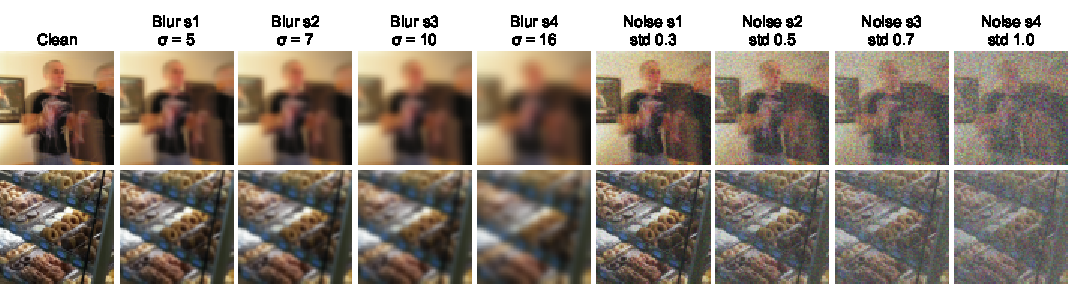
\includegraphics[width=\textwidth]{figures/fig1_degradations.pdf}
\caption{Two POPE images under the nine conditions, shown at the model's 336\,px input size. Blur is parameterised by $\sigma$ (px) and noise by its standard deviation on a $[0,1]$ intensity scale.}
\label{fig:degr}
\end{figure}

\subsection{Baseline and VCD}
Decoding is greedy, so POPE's one-word answer is fixed by the first generated token. We summarise each question by its first-token margin $m=\ell(\text{Yes})-\ell(\text{No})$; the baseline answers ``yes'' iff $m>0$. VCD replaces the logits by
\begin{equation}
s(y)=(1+\alpha)\,\ell(y\mid v,x)-\alpha\,\ell(y\mid v',x),
\label{eq:vcd}
\end{equation}
and masks every token whose probability under $v$ is below $\beta$ times the top probability. Here $v'$ is $v$ after forward diffusion to step $T$~\citep{ho2020ddpm}; we use $\alpha{=}1$, $\beta{=}0.1$, $T{=}999$. The mask can \emph{force} the answer: if ``No'' is implausible, VCD answers ``Yes'' whatever the contrast says.

\subsection{Evaluation protocol}\label{sec:protocol}
All methods are scored by one shared implementation (\code{fix\_eval/common.py}).

\paragraph{DEV/TEST split} The 500 images are split once (seed 0) into 100 DEV and 400 TEST images, giving 2{,}400 TEST questions per condition $\times$ split cell. Every hyperparameter ($\alpha$, views, layer, threshold) is chosen on DEV by its mean over all 27 cells, so each method has one global setting and is never told how degraded an image is. All reported numbers are on TEST.

\paragraph{Discrimination versus bias} AUROC of a method's first-token score measures how well it ranks present above absent objects, independent of the threshold. The \emph{matched-threshold baseline} thresholds the baseline margin so that its yes-ratio equals the method's: it is what a pure bias shift achieves, and a genuine improvement must beat it in F1.

\paragraph{Decision-preserving AUROC} Masked methods output $\pm\infty$ for forced answers---60--70\% of VCD's answers are forced---and ranking these as ties penalises the method arbitrarily. We rank forced answers among themselves by the real-branch margin, which keeps the ranking consistent with the decisions actually made, and also report the unmasked score.

\paragraph{Uncertainty} We use 95\% paired bootstrap intervals over questions (500 resamples)~\citep{efron1993bootstrap} and count the cells whose interval lies entirely above or below zero.

\subsection{Modifications investigated}
\Cref{tab:methods} lists the modifications the team investigated, grouped by the idea behind each. Stage~2 (\cref{sec:stage2}) motivated the first two groups: on clean images VCD's ``blind'' image still separates present from absent objects with AUROC 0.69, so subtracting it also subtracts evidence. The zero and shuffle hooks remove visual content inside the network; the phase-scrambled null removes it in pixel space while keeping the input's amplitude spectrum, so a blurred input yields a blurry, object-free texture (\cref{fig:nulls}). Fix~B restores the input with a small denoising autoencoder~\citep{vincent2008dae} (a 7.2M-parameter U-Net trained on COCO train2014, disjoint from POPE's val2014 images) and then decodes the restored image with the baseline (B0) or VCD (B1). RITUAL was re-implemented from the paper and DeCo ported from its official \code{deco\_greedy\_search}, verified by a CPU test against a line-by-line copy of the official logic. In the layer-routing experiments, a DoLa-style router that picks the layer of maximum Jensen--Shannon divergence from the final layer~\citep{chuang2024dola} was tried first and then replaced by entropy-weighted routing of the first token and by an entropy-based early exit; all three are scored offline from the logged per-layer logits.

\begin{table}[t]
\centering\small
\caption{Modifications investigated. ``Passes'' counts image forward passes per question (baseline: 1).}
\label{tab:methods}
\begin{tabularx}{\textwidth}{@{}l l X c@{}}
\toprule
Idea & Method (owner) & What changes & Passes\\
\midrule
\multirow{2}{*}{Blinder negative} & Zero-hook VCD (Akshay) & Contrast branch receives 576 zeroed visual tokens & 2\\
 & Shuffle-hook VCD (Akshay) & Contrast branch receives randomly permuted patch embeddings & 2\\
\addlinespace
\multirow{2}{*}{Content-free null} & Phase null (Sanjana) & Contrast image keeps the amplitude spectrum, randomises phase~\citep{oppenheim1981phase} & 2\\
 & Mean null (Sanjana) & Control: contrast image is the per-channel mean & 2\\
\addlinespace
Restoration & Fix B (Arushi) & DAE-restored input, decoded by the baseline (B0) or VCD (B1) & 1 / 2\\
\addlinespace
Extra views & RITUAL~\citep{woo2024ritual} (Sanjana) & $p(y|v)+\alpha\,p(y|T(v))$ with a random transform $T$; also six views & 2 (7)\\
\addlinespace
\multirow{2}{*}{Layer readout} & DeCo~\citep{wang2025deco} (Sanjana) & Final logits $+\,\alpha\,p_{\max}\cdot$ logits of the most confident layer in 20--28 & 1\\
 & Entropy routing (Akshay) & First token from the $K$ lowest-entropy layers in 18--30, weighted by $\mathrm{softmax}(-H/T)$; also an entropy-based early exit & 1\\
\addlinespace
\rowcolor{ours} & \textbf{\ours{} (Sanjana)} & Mean Yes--No margin over views at a DEV-chosen layer (\cref{sec:viewlayer}) & 5\\
\rowcolor{ours} \multirow{-2}{*}{Views $\times$ layer} & \ours+DAE (Sanjana) & The same, with the DAE-restored image as a sixth view & 6\\
\addlinespace
\rowcolor{ours} & \textbf{Clean-teacher probe (Akshay)} & Linear probe on the last-token hidden state, trained on the model's own clean-image answers (\cref{sec:probe}) & 1\\
\rowcolor{ours} \multirow{-2}{*}{Learned readout} & Probe $\times$ views (Akshay) & The probe's score averaged over \ours{}'s views (and the DAE view) & 5--6\\
\bottomrule
\end{tabularx}
\end{table}

\subsection{\ours{}: a view \texorpdfstring{$\times$}{x} layer readout}\label{sec:viewlayer}
\ours{} combines the two signals that our Phase~2 runs found to survive degradation (\cref{sec:all}): in the RITUAL ablation a slightly blurred copy of a noisy image raised AUROC, acting as a free denoiser, and in the DeCo layer analysis the margin read out at layer $\approx$20 separated present from absent objects better than the final layer, increasingly so with severity. DeCo's mixing weight $\alpha p_{\max}$ is too small to exploit the latter, and RITUAL uses only the final layer.

For a view set $V\subseteq\{\text{original},\text{ blur }\sigma{=}1,2,3\text{ px},\text{ horizontal flip}\}$, applied to the degraded image at native resolution, and a decoder layer $L$, the score is the mean Yes--No margin of layer $L$ read out through the final RMSNorm and LM head, as in DoLa and DeCo (\cref{fig:method}):
\begin{equation}
s(q)=\frac{1}{|V|}\sum_{u\in V}\big(w_{\text{Yes}}-w_{\text{No}}\big)^{\!\top}\,\mathrm{RMSNorm}\big(h_L(u,q)\big),\qquad \hat y=\text{``yes''}\iff s(q)>t,
\label{eq:viewlayer}
\end{equation}
where $h_L$ is the hidden state at the last prompt position and $w$ are rows of the LM head. $V$ and $L$ maximise mean DEV AUROC over nine candidate view sets and layers 12--32; $t$ maximises mean DEV F1. Because $t$ is tuned, the baseline also receives its own DEV-tuned threshold. All views share one batched forward pass. Two ablations are selected the same way: \emph{layer-only} (original image, best layer) and \emph{views-only} (best views, final layer).

\begin{figure}[t]
\centering
\begin{tikzpicture}[
  font=\small, >={Stealth[length=5pt]},
  box/.style={draw=ink2!60, rounded corners=3pt, fill=boxgray, align=center, inner sep=5pt},
  thumb/.style={inner sep=0pt, draw=white, line width=0.6pt}]
  % ---- input
  \node[thumb] (in) at (0,0) {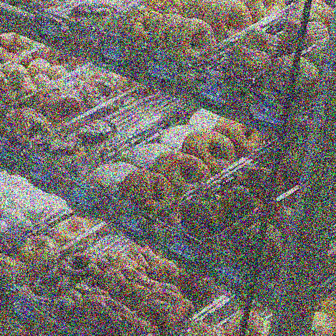
\includegraphics[width=2.3cm]{figures/vl_input.png}};
  \node[below=3pt of in, align=center, font=\footnotesize] {degraded input\\(noise s3)};
  % ---- five views (column), labels to the right
  \foreach \n/\f/\t [count=\k] in {v1/orig/original, v2/blur1/blur $\sigma{=}1$, v3/blur2/blur $\sigma{=}2$, v4/blur3/blur $\sigma{=}3$, v5/hflip/h-flip} {
    \node[thumb] (\n) at (3.3, {1.9-(\k-1)*0.95}) {\includegraphics[width=0.88cm]{figures/vl_\f.png}};
    \node[font=\scriptsize, anchor=west] (l\n) at ($(\n.east)+(0.08,0)$) {\t};
  }
  \draw[->, ink2] (in.east) -- ($(v3.west)+(-0.15,0)$);
  % collector bracket
  \draw[ink2] ($(v1.east)+(1.45,0)$) -- ($(v5.east)+(1.45,0)$);
  \foreach \n in {v1,v2,v3,v4,v5} \draw[ink2] ($(\n.east)+(1.30,0)$) -- ($(\n.east)+(1.45,0)$);
  % ---- LLaVA block with 32 decoder layers (16 bars drawn)
  \node[box, minimum height=4.6cm, minimum width=2.7cm] (llava) at (7.55,0) {};
  \node[font=\footnotesize\bfseries, anchor=north] at ($(llava.north)+(0,-0.05)$) {LLaVA-1.5-7B};
  \node[font=\scriptsize, ink2, anchor=north] at ($(llava.north)+(0,-0.42)$) {32 decoder layers};
  \foreach \i in {0,...,15} \fill[ink2!22] ($(llava.center)+(-0.75,-1.75+\i*0.19)$) rectangle ++(1.5,0.13);
  \fill[accent] ($(llava.center)+(-0.75,-1.75+9*0.19)$) rectangle ++(1.5,0.13);
  \node[font=\scriptsize, ink2, anchor=east] at ($(llava.center)+(-0.8,-1.685)$) {1};
  \node[font=\scriptsize, ink2, anchor=east] at ($(llava.center)+(-0.8,-1.685+15*0.19)$) {32};
  \node[font=\scriptsize\bfseries, accent, anchor=east] at ($(llava.center)+(-0.8,-1.685+9*0.19)$) {20};
  % batched views enter at the bottom (input embeddings)
  \draw[->, ink2] ($(v3.east)+(1.45,0)$) -- ++(0.35,0) |- ($(llava.center)+(-1.35,-1.95)$) -- ($(llava.west)+(0,-1.95)$);
  \node[font=\scriptsize, ink2, anchor=north] at ($(llava.west)+(-0.62,-1.98)$) {batch of 5};
  % ---- readout and decision
  \node[box, text width=4.4cm, anchor=west] (ro) at ($(llava.east)+(0.9,0.75)$)
     {\textbf{Read out layer 20}\\[2pt]\footnotesize $(w_{\mathrm{Yes}}-w_{\mathrm{No}})^{\top}\,\mathrm{RMSNorm}(h_{20})$\\ Yes--No margin of each view};
  \node[box, text width=4.4cm, below=0.55cm of ro] (avg) {\textbf{Average over views}\\[2pt]\footnotesize answer ``Yes'' iff $s(q)>t$};
  \draw[->, accent, thick] ($(llava.center)+(0.75,-1.685+9*0.19)$) -- ($(llava.center)+(1.6,-1.685+9*0.19)$) |- (ro.west);
  \draw[->, ink2] (ro) -- (avg);
\end{tikzpicture}
\caption{\ours{}. The degraded image and four light variants are encoded in one batched forward pass. Instead of the final layer, the Yes--No margin is read out at decoder layer 20 for every view and averaged. Views, layer and threshold are chosen on DEV images only.}
\label{fig:method}
\end{figure}

\paragraph{Disclosure} The idea of a blur view came from the RITUAL ablation, which we had inspected on TEST images. Every \emph{choice}---views, layer and threshold---was made on DEV images only, but the candidate list was informed by those earlier results.

\subsection{Probe readouts}\label{sec:probe}
\ours{} still reads a fixed direction, $w_{\text{Yes}}-w_{\text{No}}$, out of the hidden state. To ask how much of the answer the hidden state actually contains, we replace that direction by a learned one. Let $z(q)$ be the standardised last-prompt-position hidden state for question $q$ (layer 24, or layers 16 and 24 concatenated). A probe is a logistic regression
\begin{equation}
s_{\text{probe}}(q)=w^{\top}z(q)+b,\qquad \hat y=\text{``yes''}\iff s_{\text{probe}}(q)>t .
\label{eq:probe}
\end{equation}
It needs no extra forward pass. We fit it on the 9{,}234 distinct DEV questions of all nine conditions, with two kinds of label:
\begin{itemize}
\item \textbf{Gold probe:} the POPE annotation. This measures how much of the answer is linearly decodable, an upper bound for any single-pass readout of this kind.
\item \textbf{Clean-teacher probe:} no human label. Each degraded DEV question is labelled with the model's \emph{own} answer to the same question on the clean version of the image, $\mathbb{1}[m_{32}(\text{clean})>0]$. These labels agree with POPE on 89.3\% of DEV questions, which caps what the teacher can learn.
\end{itemize}
The layer set and the L2 strength are chosen by 5-fold cross-validation on DEV, grouped by image so that no image is scored by a probe that saw it (layer 24 and $C{=}10^{-3}$ for the gold probe; layers 16 and 24 and $C{=}10^{-4}$ for the clean teacher), and $t$ maximises mean DEV F1. The clean teacher therefore uses DEV labels only to choose among a few layer sets and values of $C$, all within 0.01 of each other in CV AUROC, and to set $t$, just as \ours{} uses them to choose its views, layer and threshold. Its weights see no label.

\paragraph{Probe $\times$ views} The probe can replace \ours{}'s layer-20 readout in \cref{eq:viewlayer}, so that the score is the mean of $s_{\text{probe}}$ over the views. The probe is \emph{not} refit on the views. We report \ours{}'s own five views, those plus the DAE-restored image (the views of \ours+DAE), and, separately, the best of all 63 subsets of these six images, selected on out-of-fold DEV scores. \emph{Disclosure:} this combination was motivated by a pilot on the two s4 conditions in which we inspected TEST numbers; the full evaluation fixes every choice on DEV.

% -------------------------------------------------------------------------------------
\section{Experiments and results}

\subsection{Reproducing VCD on clean images}\label{sec:repro}
Before testing degraded inputs we verified our implementation: the noise function is bit-identical to the official code for the same random stream, and the metric code matches theirs exactly. With $T{=}999$, VCD lands within 0.5 F1 of the paper on every split and the baseline within 0.25 (\cref{tab:repro}); greedy results on the random split match the paper's appendix to within 0.1 on every metric. At the code default $T{=}500$ the gain roughly halves, which explains several open reproduction issues on the official repository; all later experiments use $T{=}999$. Even on clean images most of VCD's gain comes from saying ``yes'' more often (yes-ratio 39--44\% $\to$ 46--52\%).

\begin{table}[h]
\centering\small
\caption{POPE F1 (\%) on clean images with sampling (temperature 1); mean $\pm$ std over three seeds, 3{,}000 questions per split.}
\label{tab:repro}
\begin{tabular}{@{}lccccc@{}}
\toprule
Split & Baseline (ours) & Baseline (paper) & VCD, $T{=}500$ (ours) & VCD, $T{=}999$ (ours) & VCD (paper)\\
\midrule
Random      & 81.19 $\pm$ 0.45 & 81.33 & 83.53 $\pm$ 0.30 & \textbf{87.09} $\pm$ 0.25 & 87.16\\
Popular     & 80.20 $\pm$ 0.78 & 80.06 & 82.48 $\pm$ 0.81 & \textbf{85.48} $\pm$ 0.33 & 85.06\\
Adversarial & 77.81 $\pm$ 0.29 & 77.57 & 79.62 $\pm$ 0.27 & \textbf{81.77} $\pm$ 0.31 & 81.33\\
\bottomrule
\end{tabular}
\end{table}

\subsection{VCD on degraded images}\label{sec:stage2}
\Cref{tab:stage2} compares the greedy baseline and VCD on TEST images.

\paragraph{VCD's F1 gain grows with severity} It rises from $+1.5$ on clean images to $+18.6$ at blur s4 and $+18.9$ at noise s4 (over all 500 images: $+1.2$, $+19.5$, $+20.1$, every degraded cell significant). Measured by F1, the hypothesis that VCD stops helping on degraded images is refuted.

\paragraph{But the gain is a threshold shift} Degradation pushes LLaVA toward ``no'': its yes-ratio falls from 41\% to 16--17\% at s4 while precision stays near 87--94\% and recall collapses. VCD pushes back toward ``yes'', and the matched-threshold baseline equals or beats VCD's F1 in every condition. The team's Stage~2 analysis had found VCD's AUROC below the baseline's in all 27 cells by 0.016--0.054; re-scored with the decision-preserving rule, that drop is almost entirely a tie artefact. Ranked fairly, VCD is within 0.005 of the baseline everywhere (mean $-0.0024$), and its unmasked score is slightly \emph{better} at s4.

\paragraph{The predicted mechanism is nevertheless real} The Jensen--Shannon divergence between the branches halves under degradation (0.135 $\to$ 0.066 at blur s4), and the discriminative part of the contrast---its mean on present minus absent objects---falls from 3.79 to 1.83. For absent objects the contrast even turns positive ($-0.38\to+1.07$ at noise s4). The contrast loses image information as predicted, but its large constant push toward ``yes'' happens to correct the degradation-induced bias toward ``no''.

\begin{table}[t]
\centering\small
\setlength{\tabcolsep}{5pt}
\caption{Greedy baseline vs VCD ($\alpha{=}1$, $\beta{=}0.1$, $T{=}999$) on TEST images, mean of three splits. \emph{Matched}: baseline thresholded to VCD's yes-ratio. $^\dagger$Original Stage~2 analysis (all 500 images, forced answers ranked as ties).}
\label{tab:stage2}
\begin{tabular}{@{}l ccc cc cccc@{}}
\toprule
 & \multicolumn{3}{c}{F1 (\%)} & \multicolumn{2}{c}{Yes-ratio (\%)} & \multicolumn{4}{c}{AUROC}\\
\cmidrule(lr){2-4}\cmidrule(lr){5-6}\cmidrule(l){7-10}
Condition & Base & VCD & Matched & Base & VCD & Base & VCD, ties$^\dagger$ & VCD, dec.-pres. & VCD, unmasked\\
\midrule
Clean    & 84.2 & 85.7 & \textbf{86.8} & 40.8 & 49.2 & .940 & .921 & .935 & .925\\
\addlinespace
Blur s1  & 75.9 & 82.3 & \textbf{83.0} & 34.3 & 47.4 & .907 & .884 & .904 & .897\\
Blur s2  & 70.6 & 79.0 & \textbf{79.4} & 31.0 & 45.3 & .877 & .855 & .875 & .871\\
Blur s3  & 61.0 & 73.1 & \textbf{73.4} & 25.2 & 40.6 & .836 & .800 & .834 & .833\\
Blur s4  & 41.1 & 59.7 & 59.7 & 15.5 & 30.9 & .750 & .708 & .749 & .756\\
\addlinespace
Noise s1 & 76.4 & 81.9 & \textbf{82.6} & 34.9 & 46.6 & .910 & .889 & .906 & .899\\
Noise s2 & 69.7 & 78.0 & \textbf{78.7} & 30.3 & 45.9 & .878 & .851 & .874 & .871\\
Noise s3 & 58.4 & 72.5 & \textbf{72.6} & 23.7 & 43.3 & .823 & .796 & .821 & .827\\
Noise s4 & 43.8 & 62.7 & \textbf{62.8} & 17.0 & 38.2 & .737 & .708 & .737 & .748\\
\bottomrule
\end{tabular}
\end{table}

\subsection{Comparison of all modifications}\label{sec:all}
\Cref{tab:all} scores every method on the same TEST images. Every method that keeps the final-layer readout of the original image barely changes discrimination: mean $\Delta$AUROC stays within $\pm0.005$, F1 rarely beats the matched-threshold baseline, and F1 differences between methods mostly track their yes-ratios. The zero hook is indistinguishable from the baseline and the shuffle hook is significantly \emph{worse} in 26 cells, as is the phase null in 17; RITUAL as published lowers F1 under degradation (blur s4: $41.1\to31.2$); its six-view variant gives the most consistent final-layer AUROC gain (15 cells) but an even lower F1. Entropy routing as run leaves AUROC unchanged ($-0.0003$), and its best DEV setting gains only $+0.005$. Large and consistent gains come only from methods that change the input (restoration on noise, extra views) or leave the final-layer Yes/No readout (layer 20, probes).

\begin{table}[t]
\centering\small
\setlength{\tabcolsep}{4pt}
\caption{All methods on TEST images (27 condition $\times$ split cells). Sig.\ \up/\dn: cells whose 95\% bootstrap interval lies above/below zero, against the baseline (AUROC) or the matched-threshold baseline (F1). F1 of the rows marked $^\star$ uses DEV-tuned thresholds and is directly comparable among them; other rows use their own decision rule. $^\P$Noise cells only (12): the DAE returns blurred and clean images unchanged, so on those cells B0 equals the baseline and B1 equals VCD. CT: clean-teacher. $^\S$Scored from per-layer logs regenerated on a second GPU (RTX 4500 Ada, Transformers 5); the baseline reproduces to three decimals in AUROC and within 0.3 in F1.}
\label{tab:all}
\begin{tabular}{@{}l c c cc ccc cc@{}}
\toprule
 & & Mean & \multicolumn{2}{c}{Sig.\ \up\,/\,\dn} & \multicolumn{3}{c}{AUROC} & \multicolumn{2}{c}{F1 (\%)}\\
\cmidrule(lr){4-5}\cmidrule(lr){6-8}\cmidrule(l){9-10}
Method & Passes & $\Delta$AUROC & AUROC & F1 & Clean & Blur s4 & Noise s4 & Blur s4 & Noise s4\\
\midrule
Baseline (threshold 0)        & 1 & --       & --     & --     & .940 & .750 & .737 & 41.1 & 43.8\\
Baseline (DEV threshold)$^\star$ & 1 & --    & --     & --     & .940 & .750 & .737 & 67.9 & 68.8\\
VCD                           & 2 & $-.0024$ & --     & --     & .935 & .749 & .737 & 59.7 & 62.7\\
\addlinespace
Zero-hook VCD$^\S$            & 2 & $-.0005$ & 1/18   & 0/0    & .940 & .750 & .737 & 40.6 & 43.2\\
Shuffle-hook VCD$^\S$         & 2 & $-.0032$ & 0/26   & 0/10   & .936 & .747 & .735 & 39.6 & 43.5\\
Phase null ($\alpha{=}.25$)   & 2 & $-.0008$ & 2/17   & 1/1    & .939 & .749 & .737 & 47.3 & 51.2\\
Mean null ($\alpha{=}.25$)    & 2 & $+.0003$ & 11/0   & 1/0    & .940 & .751 & .738 & 50.2 & 53.7\\
\addlinespace
Fix B0: DAE + baseline$^\P$   & 1 & $+.047$  & 12/0   & --     & .940 & .750 & .836 & 41.1 & 62.1\\
Fix B1: DAE + VCD$^\P$        & 2 & $+.041$  & 9/0    & --     & .935 & .749 & .830 & 59.7 & 71.4\\
\addlinespace
RITUAL (paper, $\alpha{=}3$)  & 2 & $-.0022$ & 0/6    & 0/5    & .939 & .750 & .735 & 31.2 & 35.0\\
RITUAL (DEV $\alpha{=}0.5$)   & 2 & $+.0006$ & 2/0    & 3/0    & .941 & .751 & .739 & 37.3 & 40.2\\
RITUAL, 6 views (DEV $\alpha{=}5$) & 7 & $+.0025$ & 15/0 & 4/0  & .942 & .751 & .743 & 28.8 & 30.7\\
\addlinespace
DeCo (paper, $\alpha{=}0.6$)  & 1 & $+.0008$ & 13/1   & 0/1    & .940 & .752 & .738 & 50.9 & 54.1\\
DeCo (DEV $\alpha{=}1.5$)     & 1 & $+.0008$ & 12/1   & 5/1    & .940 & .752 & .738 & 52.9 & 56.3\\
Entropy routing (as run)$^\S$ & 1 & $-.0003$ & 3/7 & 1/0 & .936 & .753 & .739 & 59.5 & 62.3\\
Entropy routing (DEV)$^{\star\S}$ & 1 & $+.0048$ & 17/0 & 1/2 & .941 & .762 & .741 & 67.5 & 67.8\\
\addlinespace
Layer 20 only$^\star$         & 1 & $+.0133$ & 25/0   & 3/1    & .943 & .779 & .754 & 67.5 & 67.7\\
Views only$^\star$            & 5 & $+.0151$ & 15/0   & 11/0   & .941 & .753 & .804 & 67.9 & 73.6\\
\rowcolor{ours}\textbf{\ours{}}$^\star$ & 5 & $+.0277$ & 26/0 & 10/0 & .945 & .782 & .817 & 68.6 & 73.9\\
\rowcolor{ours}\ours+DAE$^\star$ & 6 & $+.0315$ & 26/0 & 12/0 & .945 & .782 & .833 & 66.9 & 75.5\\
\addlinespace
\rowcolor{ours}\textbf{CT probe}$^{\star\S}$ & 1 & $+.0383$ & 26/0 & 21/0 & .949 & .830 & .801 & 76.4 & 73.9\\
\rowcolor{ours}\textbf{CT probe $\times$ \ours{} views}$^{\star\S}$ & 5 & $+.0491$ & 26/0 & 21/0 & .949 & .832 & .852 & 77.1 & 77.7\\
Gold probe$^{\star\S}$ & 1 & $+.0503$ & 26/0 & 25/0 & .952 & .848 & .820 & 77.7 & 75.2\\
\bottomrule
\end{tabular}
\end{table}

\subsection{ViewLayer results and ablation}\label{sec:vl}
On DEV the selected setting was all five views read out at \textbf{layer 20} (mean DEV AUROC 0.879 vs 0.857 for the baseline); layer 19 was a close second, and the best single-view layer was also 20 (\cref{fig:layers}b). On TEST (\cref{fig:auroc}), \ours{}'s AUROC is significantly above the baseline's in 26 of 27 cells---the exception, clean/adversarial, has an interval touching zero---and the gain grows with severity: $+0.005$ on clean images, $+0.032$ at blur s4 and $+0.080$ at noise s4 (95\% intervals $+0.062$ to $+0.094$ across splits).

\begin{figure}[t]
\centering
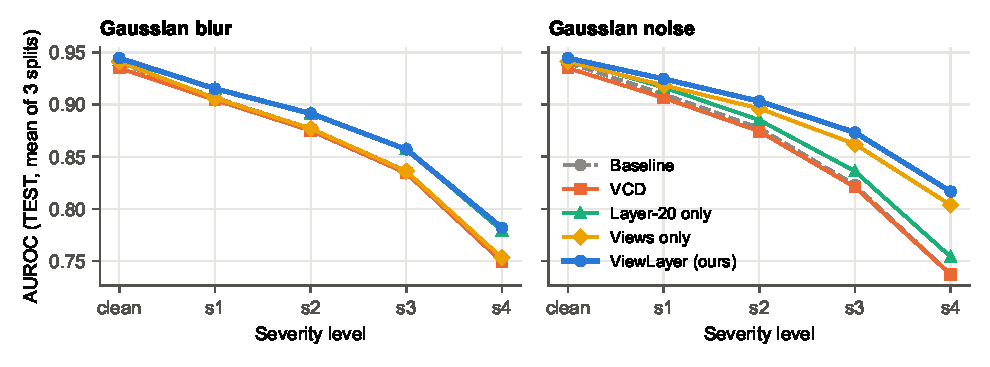
\includegraphics[width=\textwidth]{figures/fig2_auroc_severity.pdf}
\caption{TEST AUROC against severity (mean of three splits). The layer-20 readout accounts for the gain on blur and the blurred views for the gain on noise; \ours{} combines both.}
\label{fig:auroc}
\end{figure}

\paragraph{Ablation} The two components address different degradations. Layer 20 alone provides nearly all of the gain on blur (blur s4: .779 vs .782) but little on noise; the views alone provide most of the gain on noise (noise s4: .804) and nothing on blur (.753), since blurring an already blurred image adds no information. Their mean gains ($+0.013$ and $+0.015$) add up to \ours{}'s $+0.028$. \Cref{fig:layers}a shows why the layer helps: the per-layer AUROC peaks around layers 19--20, and the advantage over layer 32 grows from $+0.003$ on clean images to $+0.029$ at blur s4.

\begin{figure}[t]
\centering
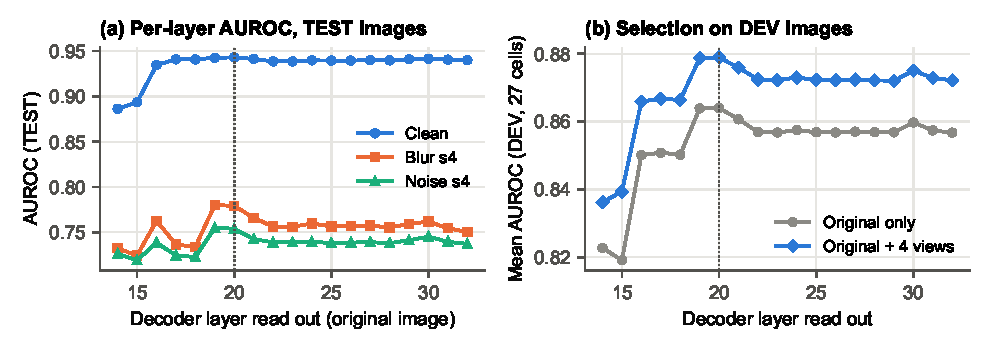
\includegraphics[width=\textwidth]{figures/fig3_layers.pdf}
\caption{(a) TEST AUROC of the Yes--No margin read out at each decoder layer from the original image. (b) DEV selection: mean DEV AUROC over all 27 cells against layer, with and without the four added views.}
\label{fig:layers}
\end{figure}

\paragraph{Operating points} \Cref{tab:op} decomposes F1 into precision, recall and false-positive rate (absent objects answered ``yes'', i.e.\ hallucinations). Against the baseline with an equally tuned threshold, \ours{} improves F1 by $+1.3$ points on average and by $+3.4/+5.1$ at noise s3/s4, where it is better on precision, recall \emph{and} false-positive rate simultaneously---so the gain is not a bias shift. It beats the threshold-matched baseline significantly in 10 cells and is never significantly worse.

\begin{table}[t]
\centering\small
\caption{Operating points on TEST images (\%, mean of three splits). Precision, recall and false-positive rate (FPR) follow exactly from F1 and the yes-ratio because every cell is balanced. Full results: \cref{app:full}.}
\label{tab:op}
\begin{tabular}{@{}l ccccc c ccccc@{}}
\toprule
 & \multicolumn{5}{c}{Blur s4} & & \multicolumn{5}{c}{Noise s4}\\
\cmidrule(lr){2-6}\cmidrule(l){8-12}
Method & Yes & Prec. & Rec. & FPR & F1 & & Yes & Prec. & Rec. & FPR & F1\\
\midrule
Baseline (threshold 0)   & 15.5 & 87.4 & 26.9 & 4.0  & 41.1 & & 17.0 & 86.8 & 29.3 & 4.6  & 43.8\\
Baseline (DEV threshold) & 43.1 & 73.6 & 63.1 & 23.1 & 67.9 & & 53.4 & 66.8 & 71.0 & 35.7 & 68.8\\
VCD                      & 30.9 & 78.7 & 48.2 & 13.5 & 59.7 & & 38.2 & 73.0 & 55.2 & 21.2 & 62.7\\
\rowcolor{ours}\textbf{\ours{}} & 43.6 & \textbf{74.0} & \textbf{64.1} & 23.1 & \textbf{68.6} & & 56.3 & \textbf{70.1} & \textbf{78.3} & 34.2 & \textbf{73.9}\\
\bottomrule
\end{tabular}
\end{table}

\subsection{Probe readouts}\label{sec:proberes}
\paragraph{The answer is in the hidden state} The gold probe on a single forward pass raises AUROC in 26 of 27 cells (mean $+0.050$, \cref{tab:all}) and beats the matched-threshold baseline's F1 in 25. The evidence is there even in the final layer: a probe on the layer-32 state reaches .845 at blur s4 and .817 at noise s4, where the Yes--No margin read from the same state gives .750 and .737. Probe accuracy is flat from layer 12 to 32 (mean $\Delta$AUROC $+0.046$ to $+0.050$), so the gain does not depend on choosing a layer. A probe that sees only the identity of the queried object, and no image, scores .704 in every condition, so the probe is not substituting an object prior for the image.

\paragraph{A label-free, single-pass alternative} The clean-teacher probe raises AUROC in 26 of 27 cells (mean $+0.038$) and beats the matched-threshold baseline's F1 in 21, with one forward pass. On average this exceeds \ours{} ($+0.028$, five passes); it is far better on blur (s4: .830 vs .782) and worse on heavy noise (s4: .801 vs .817). It transfers across degradation types: trained on clean and blurred DEV images only, it still gains $+0.035$ on the unseen noise cells (12/0 significant); trained on clean and noisy images, $+0.041$ on unseen blur (12/0). It also knows when it is unsure. When each method abstains on its least confident questions, the area under the risk--coverage curve falls from 0.131 (DEV-tuned baseline) to 0.097, and accuracy on the half of questions it is most confident about rises from 85.3\% to 90.6\%.

\paragraph{Noise sets a single-pass ceiling} At noise s4 no single-pass readout we tried exceeded .82: probes at one or several layers, probes on object-token and query-pooled image-token states, and the patch-level logit-lens score of \citet{jiang2025interpreting} (.649; no gain when fused with the baseline). \ours{}'s views reach .817 without training, while on blur the probe leaves \ours{} far behind.

\begin{table}[t]
\centering\small
\setlength{\tabcolsep}{4pt}
\caption{Probe readouts over views (TEST, 27 cells, F1 at DEV thresholds). Sig.\ \up/\dn: cells above/below the baseline, and above/below the reference (\ours{} for rows without the DAE view, \ours+DAE for rows with it) in a paired bootstrap on identical questions. CT: clean-teacher probe (no labels in its weights); the gold probe is trained on DEV labels. Probes are fit on the original view and not refit per view; DEV views: blur $\sigma{=}2$ + flip + DAE. Scored as $^\S$ in \cref{tab:all}.}
\label{tab:probe}
\begin{tabular}{@{}l c c c c cc cc@{}}
\toprule
 & & Mean & \multicolumn{2}{c}{Sig.\ \up\,/\,\dn} & \multicolumn{2}{c}{AUROC} & \multicolumn{2}{c}{F1 (\%)}\\
\cmidrule(lr){4-5}\cmidrule(lr){6-7}\cmidrule(l){8-9}
Method & Passes & $\Delta$AUROC & vs base & vs ref. & Blur s4 & Noise s4 & Blur s4 & Noise s4\\
\midrule
\ours{} & 5 & $+.0277$ & 26/0 & ref. & .782 & .817 & 68.6 & 73.9\\
\ours+DAE & 6 & $+.0315$ & 26/0 & ref. & .782 & .833 & 66.9 & 75.5\\
\addlinespace
CT probe, 1 view & 1 & $+.0383$ & 26/0 & 16/4 & .830 & .801 & 76.4 & 73.9\\
\rowcolor{ours}CT probe $\times$ \ours{} views & 5 & $+.0491$ & 26/0 & \textbf{23/0} & .832 & .852 & 77.1 & 77.7\\
CT probe, original + DAE & 2 & $+.0510$ & 26/0 & 19/0 & .830 & .862 & 76.5 & 78.9\\
CT probe $\times$ \ours+DAE views & 6 & $+.0517$ & 26/0 & 21/0 & .832 & .863 & 76.3 & 78.7\\
CT probe, DEV views & 3 & $+.0533$ & 26/0 & 23/0 & .833 & .868 & 77.4 & 79.3\\
Gold probe, DEV views & 3 & $\mathbf{+.0634}$ & 26/0 & 26/0 & \textbf{.850} & \textbf{.881} & 75.8 & \textbf{79.9}\\
\bottomrule
\end{tabular}
\end{table}

\begin{figure}[t]
\centering
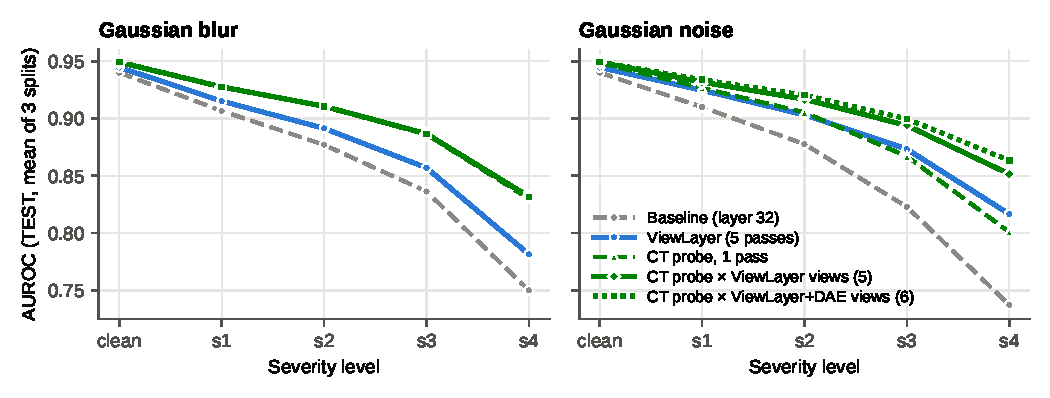
\includegraphics[width=\textwidth]{figures/fig4_probe_severity.pdf}
\caption{TEST AUROC against severity for the clean-teacher (CT) probe. On blur the three probe variants coincide: views add nothing once the readout is fixed. On noise the views supply what a single pass lacks.}
\label{fig:probe}
\end{figure}

\paragraph{Probe $\times$ views} Replacing \ours{}'s layer-20 readout by the clean-teacher probe, with \ours{}'s own five views and nothing else changed, raises AUROC above \ours{}'s in 23 of 27 cells and lowers it in none (\cref{tab:probe}, \cref{fig:probe}): blur s4 .782 $\to$ .832 and noise s4 .817 $\to$ .852, with F1 $+8.5$ and $+3.8$ points. The views add almost nothing on blur (.830 $\to$ .832) and most of the gain on noise (.801 $\to$ .852), exactly as the diagnosis predicts. The DAE-restored image is the most useful single view on noise: the probe on the original and restored images alone (two passes) reaches .862, above \ours+DAE with six passes (.833; better in 19 cells, worse in none). The subset chosen on DEV, blur $\sigma{=}2$ + flip + DAE, adds little more (.868), so the result does not hinge on the view search. With DEV labels the gold probe on the same views is the strongest method overall ($+0.063$, F1 above the matched-threshold baseline in all 27 cells).

\subsection{Failure analysis}\label{sec:fail}
\paragraph{VCD adds hallucinations along with recall} Under degradation the contrast is positive for absent objects, so VCD's false-positive rate rises from 4.6\% to 21.2\% at noise s4 while its AUROC is unchanged: its F1 gain is paid for with hallucinations that a threshold change would produce equally.

\paragraph{RITUAL amplifies the ``no'' bias} Its views are degraded too and lean ``no'' as much as the original, so adding $\alpha{=}3$ times their probability strengthens the bias (yes-ratio at blur s4: $15.5\%\to10.6\%$) and F1 drops. Individually, vertical flip, rotation, colour jitter and crop lower AUROC in most conditions; only horizontal flip (neutral) and the Gaussian-blur view, which helps noisy images ($.737\to.751$ at noise s4), do not (\cref{app:ritual}). This observation motivated \ours{}'s blur views.

\paragraph{Null images are not content-free} On its own, the phase-null branch still ranks present above absent objects with AUROC 0.56--0.58 on blurred inputs: the amplitude spectrum carries scene gist~\citep{oliva2001gist} (a savanna texture raises the prior for ``giraffe''), so subtracting it removes evidence. The mean null has AUROC 0.43, below chance, so subtracting it adds a little signal---hence its 11 small gains.

\paragraph{Blinder negatives are not blind, or not useful} The zero hook's branch is a pure text prior, identical for every image of a question; the mask fixes about 70\% of answers and on the rest a constant prior only shifts the margin, so the result equals the baseline. The shuffle hook only permutes patch embeddings, so its branch still ``sees'' the objects and subtracting it removes evidence, as with the phase null.

\paragraph{Layer routing by confidence picks confidently wrong layers} On degraded inputs the final-layer distribution is too flat for the JSD criterion to be informative; the router chose the earliest candidate layer, which produced malformed text without an end-of-sequence token and no parsable answers. Entropy weighting removed the collapse but only matched the baseline. Leaning harder on low entropy makes it worse: routing to the single lowest-entropy layer costs $-0.021$ AUROC (worse in 25 cells) and an entropy-based early exit $-0.036$ (worse in all 27). Under degradation the early layers that are most confident are confident about the language prior, not the image.

\paragraph{Where \ours{} fails} (i)~\emph{Clean images}: AUROC rises by only $+0.005$ and F1 is 0.2 below the DEV-threshold baseline. (ii)~\emph{Adversarial split}: gains are smallest (noise s4: $+4.0$ F1 vs $+6.3$ on random), because co-occurring absent objects carry the strongest prior. (iii)~\emph{Blur}: the views do not help, so the gain rests on layer 20 alone. (iv)~\emph{Operating point}: one F1-optimal global threshold gives yes-ratios of 44--62\% and false-positive rates of 23--34\% (baseline at threshold 0: 4--5\%); the DEV-tuned baseline behaves the same, so this reflects F1 tuning on balanced data rather than the score, and a hallucination-averse deployment should use a stricter threshold. (v)~\emph{Lost information}: even at .817, noise s4 AUROC stays far below clean (.945); views and layers recover evidence the model computed but ignored, not evidence the degradation destroyed.

\paragraph{Where the probes fail} (i)~\emph{Heavy noise, single pass}: the clean-teacher probe is below \ours{} at noise s3--s4 ($-0.016$ at s4); one pass of a very noisy image does not contain enough evidence. (ii)~\emph{Teacher ceiling}: the teacher's labels are wrong wherever the clean model is (10.7\% of DEV questions), which is most of its gap to the gold probe. (iii)~\emph{Clean/adversarial}: like every method here, no probe is significantly above the baseline in this cell. (iv)~\emph{Operating point}: with one global DEV threshold the teacher's yes-ratio climbs to 62--66\% at s4, against 53\% for the DEV-tuned baseline. (v)~\emph{Not training-free}: the probe is a fitted head of 8{,}192 weights, and the teacher needs clean/degraded image pairs at training time, which synthetic degradation provides but real degraded photographs would not.

% -------------------------------------------------------------------------------------
\section{Discussion}\label{sec:discussion}
\paragraph{What we learned about VCD} The original hypothesis was right about the mechanism and wrong about the outcome. Degradation does make the branches converge and drains the contrast of image information, but on POPE the dominant failure under degradation is \emph{missing} objects, and VCD's steady push toward ``yes'' compensates for it. F1 alone cannot distinguish a better decoder from a recalibrated one; we recommend reporting AUROC with a decision-preserving tie rule and a threshold-matched baseline for any decoding-time method. Without the tie rule, our own Stage~2 analysis overstated VCD's discrimination loss roughly tenfold.

\paragraph{Why \ours{} works} It exploits two sources of evidence that the final-layer readout of the original image discards. Averaging over lightly blurred views is test-time augmentation~\citep{shanmugam2021tta} that suppresses pixel noise before the encoder; the intermediate-layer readout recovers evidence that the final layers overwrite with language priors, as DeCo~\citep{wang2025deco} reported on clean images---we find this effect small on clean images but growing with degradation. Because the two sources repair different degradations, their gains add. And since \ours{} subtracts nothing, it sidesteps the failure shared by every contrastive variant we tried: there is no reliably blind image to subtract.

\paragraph{What the probes add} The probes turn \ours{}'s ablation into a diagnosis. On blur a single pass still contains the answer, but the fixed Yes/No direction reads it poorly, which agrees with \citet{li2025trainingbias}, who place the hallucination bias in the LM head rather than the hidden states. On heavy noise the evidence is partly lost before the decoder, and only a cleaner input, through blurred views or the DAE, recovers it. A probe read out over views applies both fixes. The clean teacher shows that the better readout can be learned from the model itself: its own clean-image answers are enough supervision.

\paragraph{Novelty} RITUAL and DeCo were proposed and evaluated on clean images, using only the final layer and only the original view, respectively; to our knowledge neither has been studied on degraded inputs or combined. Probes for object presence in VLMs are established (\cref{sec:related}); what we have not found in prior work is a probe distilled from the model's own clean-image answers for degraded inputs, or the separation of readout and input failures it reveals. Our contributions are a controlled study of training-free decoding under graded blur and noise, an evaluation protocol that separates discrimination from bias, well-supported negative results for blinder negatives, content-free nulls, published multi-view decoding and confidence-based layer routing, and two readouts whose gains are explained by which degradation they repair.

\paragraph{Limitations} We test one model, one benchmark and two synthetic degradations; low light, compression and motion blur are untested. All readouts score the first token and so apply to yes/no questions; free-form captioning (CHAIR~\citep{rohrbach2018chair}) would need a per-token readout. The DEV set is small (100 images), the blur-view candidate and the probe $\times$ views combination were suggested by earlier TEST observations, and the bootstrap resamples questions, which are correlated within an image, so intervals are somewhat optimistic. Rows using the DAE rely on a network trained on synthetic noise. Five batched views cost 0.33\,s per question on an A100, against 0.08\,s for the baseline and 0.16\,s for VCD; the probe adds one dot product to the baseline.

\paragraph{Future work} A per-token probe for free-form generation evaluated with CHAIR; other VLMs and real-world corruptions, where the clean teacher would need a substitute for clean/degraded pairs; and views chosen per image from an estimate of the noise level.

% -------------------------------------------------------------------------------------
\section{Conclusion}
On degraded images, VCD's large F1 gains on POPE come from recalibrating LLaVA's degradation-induced reluctance to say ``yes'', not from better visual grounding: a threshold change achieves the same, and once forced answers are ranked fairly its discrimination is unchanged. Stronger negatives, content-free nulls, RITUAL and DeCo do not change this picture. Reading the model out at layer 20 and averaging over lightly blurred views does: with every choice fixed on DEV images, \ours{} improves held-out AUROC in 26 of 27 cells and F1 by up to 5 points over an equally tuned baseline, with the largest gains under heavy noise---the setting this project set out to fix. Linear probes explain why and go further. A degraded image's hidden state still encodes most of the answer, so blur is mainly a readout failure, while heavy noise also destroys evidence that only cleaner views restore. A probe trained on the model's own clean-image answers, with no human labels, beats \ours{} on average in a single pass and, read out over \ours{}'s views, beats it in every condition.

% -------------------------------------------------------------------------------------
\section*{AI Use Statement}
\addcontentsline{toc}{section}{AI Use Statement}
We used \textbf{Claude Code} (Anthropic, Claude Opus model) as a coding and research assistant: to search the literature for training-free hallucination fixes; to implement and test the evaluation package (\code{fix\_eval}), the phase/mean nulls, the RITUAL and DeCo re-implementations and \ours{}; to submit and monitor ASPIRE jobs; to produce the analysis tables and figures; and to draft this report. We verified its outputs with 21 CPU unit tests (including a check of the DeCo port against a line-by-line copy of the official code), smoke runs before every full run, and sanity checks: the layer-32 readout reproduces the Stage~2 baseline margin (maximum difference 0.10 logits, from fp16 batching), and margins recomputed from logged logits agree with the decoded answers on 100\% of questions. References were checked against arXiv and conference pages. Errors introduced by the assistant, such as rounding probabilities to six decimals, were caught and corrected. For the layer-routing, zero/shuffle-hook and probe work, Claude Code also wrote the per-layer logging, contrast and probe pipelines and ran the local GPU queue. These were checked by re-scoring: the offline entropy routing reproduces the earlier GPU run to within 0.004 logits, the zero-hook contrast logits match the earlier \code{vcd\_zero} runs exactly, and \ours{} recomputed from the new logs matches its published AUROC (.781/.817 at s4) exactly. An error in which the assistant deleted a completed run after misreading its log was caught and the run repeated. \todo{Arushi: add the AI tools you used and how you checked them.} The team chose the research question, degradations and evaluation criteria, decided which methods to pursue or drop, ran the experiments and interpreted the results; every number reported comes from experiments the team ran.

% -------------------------------------------------------------------------------------
{\small
\setlength{\bibsep}{2pt plus 1pt}
\renewcommand{\bibsection}{\section*{References}\addcontentsline{toc}{section}{References}}
\bibliographystyle{unsrtnat}
\bibliography{refs}
}

% =====================================================================================
% APPENDIX (excluded from the page limit)
% =====================================================================================
\clearpage
\appendix
\counterwithin{table}{section}
\counterwithin{figure}{section}

\section{Reproducing the results}\label{app:repro}
\begingroup\raggedright\setlength{\parindent}{0pt}
\paragraph{Dependencies} Python 3.11; PyTorch 2.5.1 (CUDA 12.1) and torchvision; pinned packages in \code{requirements.txt} (transformers 4.46.3, accelerate 1.1.1, pillow 11.0.0, numpy 1.26.4, scipy, scikit-image, pandas, pyyaml). On ASPIRE, \code{scripts/setup\_aspire.sh} builds the conda environment. Weights are downloaded once on a login node (\code{huggingface-cli download llava-hf/llava-1.5-7b-hf}); jobs then run with \code{HF\_HUB\_OFFLINE=1}.

\paragraph{Data} Set \code{VCD\_DATA\_ROOT} and \code{VCD\_OUTPUT\_ROOT}, then run \code{python -m scripts.download\_pope} (login node; POPE questions and 500 COCO images), \code{python -m scripts.make\_degraded} (clean, blur s1--s4 and noise s1--s4 PNGs and \code{manifest.csv}) and \code{python -m scripts.contact\_sheet} (\cref{fig:degr}).

\paragraph{Baseline and VCD (Stages 0--2)} \code{python -m scripts.make\_configs stage2} writes the run configs; \code{bash scripts/submit.sh configs/stage2/} submits them; \code{python -m scripts.analyze --stage stage2} writes the comparison, diagnostic and margin tables.

\paragraph{Phase 2 methods} Each folder contains a PBS array job over the nine conditions, an analysis script that fills the folder's README and writes \code{results/<method>\_*.csv}, and CPU tests:

\begin{center}\small
\begin{tabular}{@{}ll@{}}
\toprule
Run (ASPIRE) & Analyse\\
\midrule
\code{qsub model\_fix\_2/run\_nulls.pbs} & \code{python -m model\_fix\_2.analyze}\\
\code{qsub RITUAL/run\_ritual.pbs} & \code{python -m RITUAL.analyze}\\
\code{qsub DeCo/run\_deco.pbs} & \code{python -m DeCo.analyze}\\
\code{qsub ViewLayer/run\_viewlayer.pbs} & \code{python -m ViewLayer.analyze}\\
\bottomrule
\end{tabular}
\end{center}

Adding \code{-J 4-8:4 -v LIMIT=30} to \code{qsub} runs a 30-question smoke test, and \code{python -m pytest ViewLayer/tests RITUAL/tests DeCo/tests model\_fix\_2/tests -q} runs the CPU tests. 

\paragraph{Fix B} \code{python -m scripts.download\_coco\_train} (login node) and \code{qsub -v NAME=dae\_v1 scripts/pbs/train\_dae.pbs} train the DAE; \code{python -m scripts.make\_restored} writes the restored POPE images; \code{python -m scripts.make\_configs fixb} and \code{bash scripts/submit.sh} run B0--B2; \code{python -m scripts.analyze\_fixb --test-only} scores them on the TEST images.

\paragraph{Layer routing, hooks and probes} These run on any single GPU with one forward pass per question. \code{python -m scripts.run\_layers} logs the per-layer Yes/No logits, entropies and last-token hidden states for the nine conditions; \code{python -m scripts.run\_contrast} logs the zero/shuffle-hook contrast branches. \code{python -m scripts.analyze\_layers} scores entropy routing, layer readouts and the probes; \code{python -m scripts.analyze\_contrast} the hooks; \code{python -m scripts.analyze\_selective} the risk--coverage curves. \code{bash scripts/queue\_probe\_views\_dae.sh} logs \ours{}'s views and the DAE view and runs \code{python -m scripts.analyze\_probe\_views\_dae}; \code{python Report/scripts/fig\_probe\_severity.py} draws \cref{fig:probe}.

\par\endgroup
\begin{figure}[H]
\centering
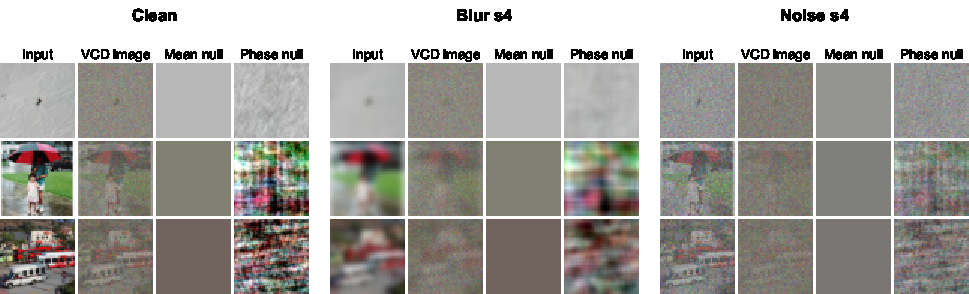
\includegraphics[width=\textwidth]{figures/fig_nulls.pdf}
\caption{Contrast images for three inputs. VCD's $T{=}999$ image still shows faint object outlines; the mean null is uniform; the phase null keeps the input's blur or graininess but no objects.}
\label{fig:nulls}
\end{figure}

\section{Per-condition ViewLayer results}\label{app:full}
\begin{table}[H]
\centering\small
\caption{TEST images, mean of three splits. VCD AUROC uses the decision-preserving rule. Per-split values with bootstrap intervals: \code{results/viewlayer\_comparison.csv}.}
\begin{tabular}{@{}l ccc cccc c@{}}
\toprule
 & \multicolumn{3}{c}{AUROC} & \multicolumn{4}{c}{F1 (\%)} & \\
\cmidrule(lr){2-4}\cmidrule(lr){5-8}
Condition & Base & VCD & \ours{} & Base (thr.\ 0) & Base (DEV thr.) & VCD & \ours{} & Yes\% \ours{}\\
\midrule
Clean    & .940 & .935 & \textbf{.945} & 84.2 & 84.7 & \textbf{85.7} & 84.5 & 61.8\\
\addlinespace
Blur s1  & .907 & .904 & \textbf{.915} & 75.9 & 83.2 & 82.3 & \textbf{83.4} & 57.9\\
Blur s2  & .877 & .875 & \textbf{.892} & 70.6 & 80.6 & 79.0 & \textbf{80.8} & 55.9\\
Blur s3  & .836 & .834 & \textbf{.857} & 61.0 & 77.3 & 73.1 & \textbf{77.8} & 52.6\\
Blur s4  & .750 & .749 & \textbf{.782} & 41.1 & 67.9 & 59.7 & \textbf{68.6} & 43.6\\
\addlinespace
Noise s1 & .910 & .906 & \textbf{.925} & 76.4 & 82.9 & 81.9 & \textbf{83.7} & 59.6\\
Noise s2 & .878 & .874 & \textbf{.903} & 69.7 & 80.5 & 78.0 & \textbf{81.7} & 58.4\\
Noise s3 & .823 & .821 & \textbf{.873} & 58.4 & 75.6 & 72.5 & \textbf{79.0} & 57.4\\
Noise s4 & .737 & .737 & \textbf{.817} & 43.8 & 68.8 & 62.7 & \textbf{73.9} & 56.3\\
\bottomrule
\end{tabular}
\end{table}

\section{RITUAL per-transform ablation}\label{app:ritual}
\begin{table}[H]
\centering\small
\caption{TEST AUROC of RITUAL with each single transform as the view ($\alpha{=}3$), mean of three splits.}
\begin{tabular}{@{}lccccccc@{}}
\toprule
Condition & Baseline & H-flip & V-flip & Rotate & Colour jitter & Gaussian blur & Crop\\
\midrule
Clean    & .940 & .941 & .937 & .938 & .939 & .939 & .936\\
\addlinespace
Blur s1  & .907 & .908 & .900 & .905 & .904 & .906 & .904\\
Blur s2  & .877 & .878 & .874 & .875 & .874 & .876 & .874\\
Blur s3  & .836 & .837 & .830 & .835 & .830 & .836 & .833\\
Blur s4  & .750 & .751 & .746 & .750 & .747 & .750 & .748\\
\addlinespace
Noise s1 & .910 & .911 & .906 & .907 & .908 & \textbf{.912} & .907\\
Noise s2 & .878 & .881 & .870 & .868 & .872 & \textbf{.883} & .875\\
Noise s3 & .823 & .824 & .816 & .815 & .817 & \textbf{.836} & .818\\
Noise s4 & .737 & .739 & .731 & .729 & .732 & \textbf{.751} & .732\\
\bottomrule
\end{tabular}
\end{table}

\end{document}
